% Editable continuation of ONED_PRL_REPRODUCTION.tex.
% Numerical macros and vector figures are refreshed by the PDF builder.
% Generated from the Fig. 2-3 comparison.json.
\newcommand{\FigTwentyThreePrimaryCount}{57}
\newcommand{\FigTwentyThreePairedCount}{57}
\newcommand{\FigTwentyThreeExtendedCheckedCount}{215}
\newcommand{\FigTwentyThreeFailedCount}{47}
\newcommand{\FigTwentyThreeSaltfreeMoment}{$50.91$}
\newcommand{\FigTwentyThreeSaltfreeEquimolar}{$38.45$}
\newcommand{\FigTwentyThreeNeutralMoment}{$21.78$}
\newcommand{\FigTwentyThreeFullResidual}{$6.02\times10^{-8}$}
\newcommand{\FigTwentyThreeChainError}{$2.33\times10^{-13}$}
\newcommand{\FigTwentyThreeContourError}{$1.98\times10^{-12}$}
\newcommand{\FigTwentyThreeMassError}{$3.55\times10^{-15}$}
\newcommand{\FigTwentyThreeCounterionMassError}{$3.55\times10^{-15}$}
\newcommand{\FigTwentyThreePairHeightDifferenceNm}{$2.85\times10^{-7}$}
\newcommand{\FigTwentyThreePairGammaDifference}{$2.90\times10^{-9}$}
\newcommand{\FigTwentyThreePairPsiDifference}{$6.81\times10^{-9}$}
\newcommand{\FigTwentyThreePairDensityDifference}{$1.90\times10^{-8}$}
\newcommand{\FigTwentyThreePairPotentialProfileDifference}{$2.71\times10^{-8}$}
\newcommand{\FigTwentyThreeMinimaRows}{%
$1$ & $50$ & $21.91$ & $-0.3661$ \\
$2$ & $0.1$ & $19.51$ & $-0.4165$ \\
$3$ & $0.03162$ & $14.11$ & $-0.5572$ \\
}
\newcommand{\FigTwentyThreeGridRows}{%
$1$ & $0$ & $8.02\times10^{-4}$ & $0.01049$ \\
$1$ & $1.00\times10^{-7}$ & $8.02\times10^{-4}$ & $0.009946$ \\
$2$ & $0.1$ & $0.00221$ & $-0.5041$ \\
$3$ & $0.01$ & $0.003446$ & $-0.3023$ \\
$3$ & $10$ & $0.001948$ & $-5.11\times10^{-5}$ \\
}

\clearpage
\pagetitle{Fig. 2: contraction and re-expansion}{figtwo}
\smallnote{Additional calculations: 1D smoothed-LDA SCFT at fixed parameters. These do not validate
the paper's full SI theory or the existing CL dynamics.}

For each $z_+=1,2,3$, 19 standard points span $10^{-7}\le\rho_b\le50\units{M}$;
validated solutions were obtained at \FigTwentyThreePrimaryCount/57 points.
Upward/downward concentration continuation and intermediate points used separate SLURM jobs.
No valence-dependent background salt concentration or height correction was fitted.

\begin{center}
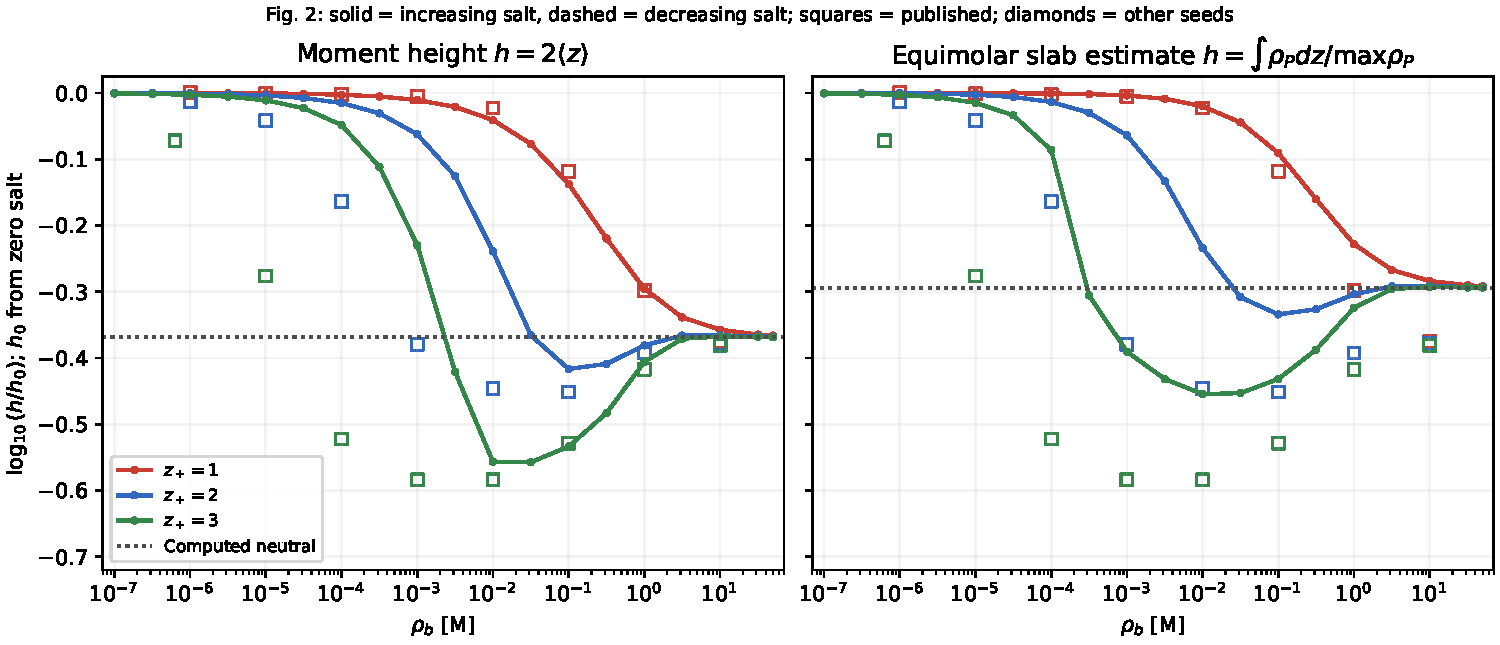
\includegraphics[width=\linewidth]{prl_comparison_figs/fig23_prl_20260907/fig2_checked.pdf}
\end{center}
\vspace{-7pt}
\smallnote{Solid/dotted: upward/downward scans. Open squares: digitized paper theory curves.
Diamonds mark points obtained only from separate initial states, if any. Experimental symbols were excluded.
Digitization uncertainty is about $0.01$ in $\log_{10}(h/h_0)$, not a statistical error.}

\subhead{Explicit height definitions and salt-free references}
\begin{equation*}
 h_{\rm m}=\frac{2\int z\rho_{\rm P}(z)\,dz}{\sigma N},\qquad
 h_{\rm eq}=\frac{\sigma N}{\max_z\rho_{\rm P}(z)},\qquad
 \int\rho_{\rm P}(z)\,dz=\sigma N=10\units{nm^{-2}}.
\end{equation*}
$h_{0,\rm m}=$\FigTwentyThreeSaltfreeMoment\,nm,
$h_{0,\rm eq}=$\FigTwentyThreeSaltfreeEquimolar\,nm were obtained by
solving $\rho_b=0$ directly. The neutral brush has moment height
\FigTwentyThreeNeutralMoment\,nm.
The paper mentions a Gibbs dividing surface without specifying the extraction procedure or reference density.
Neither definition above is therefore assumed equal to the paper's Gibbs height.

\subhead{Minimum moment heights among the 19 standard points}
\begin{tabularx}{\linewidth}{@{}Xrrr@{}}
\toprule
\rowcolor{panel}$z_+$ & $\rho_b$ [M] & $h_{\rm m}$ [nm] & $\log_{10}(h_{\rm m}/h_{0,\rm m})$ \\
\midrule
\FigTwentyThreeMinimaRows
\bottomrule
\end{tabularx}
\smallnote{These are sampled minima, not exact minima over continuous concentration. The monovalent minimum is at the scan limit.
Multivalent contraction and re-expansion occur, but the onset of contraction at low salt differs from the paper.
Changing the height definition does not produce simultaneous quantitative agreement for all three curves.}

\clearpage
\pagetitle{Fig. 3: effective charge and potential}{figthree}
\smallnote{SCFT profile observables are distinguished from direct evaluation of the paper's Eqs.~(7) and (9).}
\begin{center}
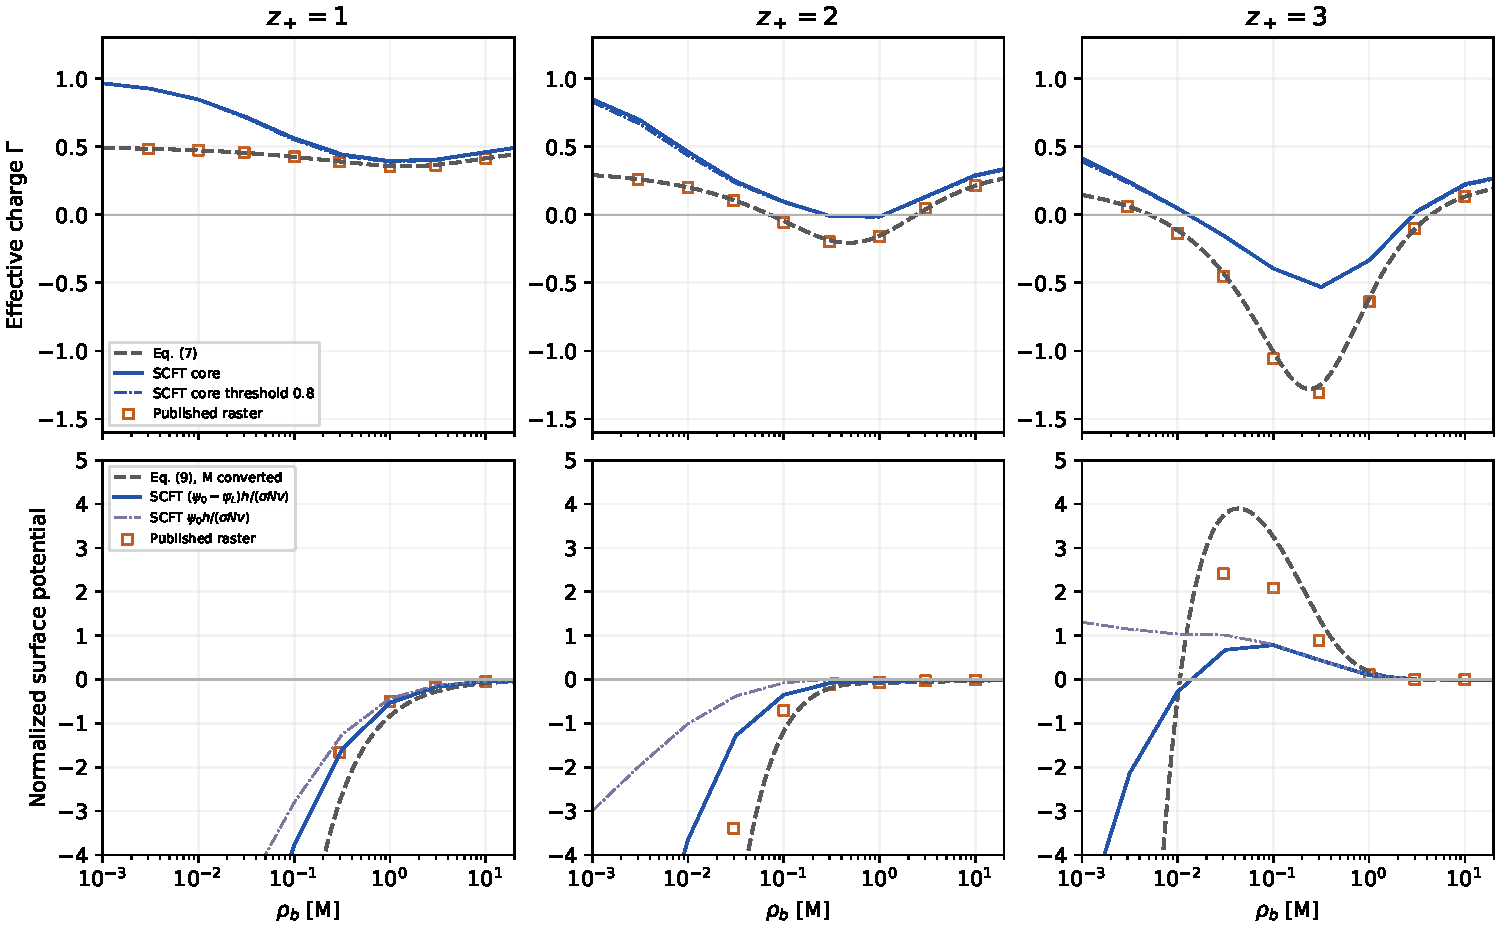
\includegraphics[width=\linewidth]{prl_comparison_figs/fig23_prl_20260907/fig3_checked.pdf}
\end{center}
\vspace{-5pt}
\smallnote{Gray dashed: analytical formulas. Squares: paper curves. Blue: SCFT.
Solid/dotted SCFT lines show upward/downward scans. Large negative potentials outside the plotting range are clipped.}

\subhead{Observables measured from SCFT}
\begin{align*}
 \Gamma(z)&=1-z_+\frac{\rho_+(z)-\rho_b}{\rho_{\rm P}(z)},
 &\overline\Gamma_c&=
 \frac{\int_{\rho_{\rm P}>c\rho_{\rm P}^{\max}}\rho_{\rm P}(z)\Gamma(z)\,dz}
 {\int_{\rho_{\rm P}>c\rho_{\rm P}^{\max}}\rho_{\rm P}(z)\,dz},\\
 \Psi_{\rm rel}&=[\psi(0)-\psi(L)]\frac{h_{\rm m}}{\sigma Nv},
 &\Psi_0&=\psi(0)\frac{h_{\rm m}}{\sigma Nv}.
\end{align*}
Both core thresholds, $c=0.5$ and $0.8$, are plotted. These explicit averages of nonuniform profiles
are not automatically equivalent to the paper's uniform-brush scaling variables.

The finite box contains a fixed number of monovalent counterions, allowing $\psi(L)\ne0$.
We therefore record both $\Psi_0$ relative to zero and the wall--far-end difference $\Psi_{\rm rel}$.
The sign of $\psi(0)$ alone does not establish charge inversion, particularly at low salt.
Wall/far-end potentials are approximated by first/last cell-center values.

\subhead{Analytical formulas and SCFT have different scopes}
SI Eq.~(S34) assumes high salt, $\rho_b\gg\rho_{\rm P}$, with negligible canonical counterion effects.
Low-salt SCFT does not satisfy these conditions.
Reproducing the analytical formulas therefore does not validate SCFT or CL.
The current LDA must be compared with the paper's nonlocal Green function/$I^{\rm ex}$ treatment.
The paper also neglects $u_{\rm P}^{\rm ex}$ for brushes; that omission alone is not an established cause of the discrepancy.

\smallnote{Among the 19 standard points, the divalent core $\Gamma$ reaches $-0.0140$, while $\Psi_{\rm rel}$
remains negative. For trivalent salt, $\Gamma_{\min}\simeq-0.5314$ and $\Psi_{{\rm rel},\max}\simeq+0.7834$.
Overcharging and potential reversal are qualitatively distinct, but the trivalent potential peak differs from the paper's value of about 2.5.}

\clearpage
\pagetitle{Checking Fig. 3 potential normalization}{figthreeunits}
\smallnote{A diagnostic of the equation--figure discrepancy. The scale factor below was not applied to SCFT results.}
The paper's Gaussian charge-spread function and Eqs.~(7), (9) were evaluated as follows.
\begin{align*}
 u(x)&=1-x\,\operatorname{erfcx}(x/\sqrt\pi),
 &u'(x)&=-\left(1+\frac{2x^2}{\pi}\right)\operatorname{erfcx}(x/\sqrt\pi)+\frac{2x}{\pi},\\
 \kappa_b^2&=4\pi\ell_B z_+(z_++1)\rho_b,
 &R&=-\frac{z_+(z_++1)\kappa_b\ell_B}{4}u'(a\kappa_b),\\
 \Gamma&=\frac{1-R}{z_++1-R},
 &\Psi_{\rm Eq.9}&=-\frac{(z_+^2-1)\Gamma+1}{z_+^2(z_++1)v\rho_b}.
\end{align*}
Parameters are $a=0.25\units{nm}$, $\ell_B=0.7\units{nm}$, and $v=1\units{nm^3}$.
The formulas use number density $\rho_b[\mathrm{nm^{-3}}]=0.6022\,\rho_b[\mathrm M]$.

\begin{center}
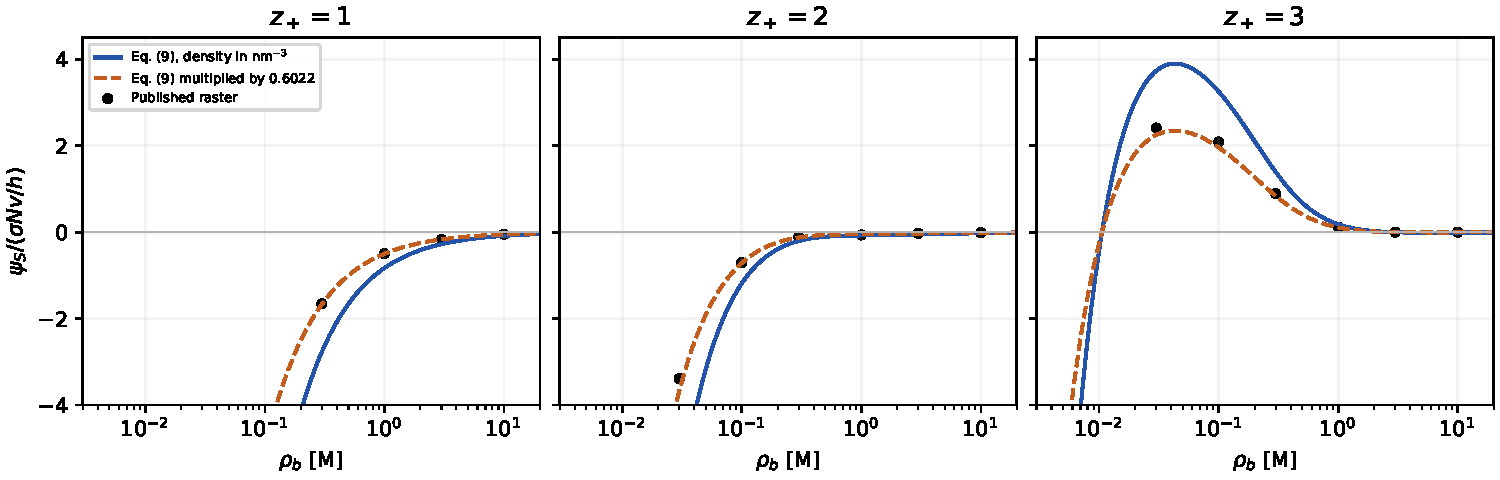
\includegraphics[width=\linewidth]{prl_comparison_figs/fig23_prl_20260907/fig3_units_check.pdf}
\end{center}
\vspace{-6pt}
\smallnote{Blue: Eq.~(9) with unit conversion. Orange dotted: that value multiplied by 0.6022, for diagnosis only.
Black dots: digitized original raster. The latter scale equals omitting the density conversion in the denominator;
it is not asserted to be the correct physical normalization.}

\subhead{The monovalent check is independent of correlation parameters}
For $z_+=1$, $\Psi_{\rm Eq.9}=-1/(2v\rho_b)$, eliminating $a,\ell_B,\Gamma$.

\begin{tabularx}{\linewidth}{@{}Xrrr@{}}
\toprule
\rowcolor{panel}$\rho_b$ [M] & Eq.~(9), converted & Paper (approx.) & Eq.~(9)$\times0.6022$ \\
\midrule
$0.3$ & $-2.7676$ & $-1.6598$ & $-1.6667$ \\
$1$ & $-0.8303$ & $-0.4985$ & $-0.5000$ \\
$3$ & $-0.2768$ & $-0.1701$ & $-0.1667$ \\
\bottomrule
\end{tabularx}

The monovalent discrepancy is consistent with the M--nm$^{-3}$ conversion factor. Multivalent discrepancies remain.
\textbf{The units/normalization connecting the paper's equations and figure require confirmation.}
The cause is not established without the authors' raw data or plotting code.
\smallnote{Source: \href{https://doi.org/10.1103/PhysRevLett.134.048101}{Duan et al., PRL 134, 048101 (2025)},
Eqs.~(7), (9), Fig.~3, and SI Eqs.~(S33), (S38). The printed SI Eq.~(S42) lacks the
$\rho_b$ denominator visible in main-text Eq.~(9); potentials were therefore evaluated from the main-text equation.}

\clearpage
\pagetitle{Numerical checks and remaining gaps}{figtwothreechecks}
\subhead{Numerical issues addressed in a separate Python research runner}
The existing real-space chain calculation also suffered floating-point underflow at low salt.
Densities differed from an independent log-space calculation by up to $0.2098\units{nm^{-3}}$,
hidden by per-bead floors and final mass normalization.
The new runner evaluates positive bond convolutions in extended precision,
using one partition function for every contour position.
Independent log-sum-exp calculations check final densities and contour consistency.

The runner adds Poisson--Boltzmann Newton updates including derivatives of canonical C normalization.
The Jacobian is tridiagonal plus a rank-one term.
For random fields (std $\simeq5$), its relative finite-difference error was $3.77\times10^{-10}$.
These changes are confined to \texttt{run\_prl\_fig23\_checked.py}.
Production FFT/C++/CUDA, CL drift, and the existing \texttt{prl\_scft.py} were unchanged in this work.

\subhead{Acceptance criteria and maximum observed errors}
\begin{tabularx}{\linewidth}{@{}Xrr@{}}
\toprule
\rowcolor{panel}Check & Required & Observed maximum \\
\midrule
Full SCFT residual & $10^{-7}$ & \FigTwentyThreeFullResidual \\
Independent chain density difference & $10^{-10}$ & \FigTwentyThreeChainError \\
Relative contour partition error & $10^{-10}$ & \FigTwentyThreeContourError \\
Polymer integral error [nm$^{-2}$] & $10^{-10}$ & \FigTwentyThreeMassError \\
Canonical C integral error [nm$^{-2}$] & $10^{-10}$ & \FigTwentyThreeCounterionMassError \\
\bottomrule
\end{tabularx}
\FigTwentyThreeExtendedCheckedCount{} extended-precision runs passed validation.
Failed attempts are excluded from successful results; their logs and checkpoints are preserved.
Across \FigTwentyThreePairedCount{} upward/downward pairs at matching concentrations,
the largest height difference is \FigTwentyThreePairHeightDifferenceNm\,nm.
The maximum full polymer density profile difference is \FigTwentyThreePairDensityDifference\,nm$^{-3}$.
This checks iterative solution consistency; it does not prove a free-energy minimum.

\subhead{Grid and box size: moment height changes [nm]}
The reference is $L=200\units{nm}$, $N_z=1600$. Grid refinement uses $N_z=3200$;
box enlargement uses $L=400\units{nm}$, $N_z=3200$.

\begin{tabularx}{\linewidth}{@{}Xrrr@{}}
\toprule
\rowcolor{panel}$z_+$ & $\rho_b$ [M] & $\Delta h$, finer grid & $\Delta h$, larger box \\
\midrule
\FigTwentyThreeGridRows
\bottomrule
\end{tabularx}
\smallnote{These are selected-point checks, not proof of $L\to\infty$ convergence for the full scan.
One failed high-salt PB residual check was rerun with a tighter inner PB tolerance.
The SCFT acceptance threshold was not relaxed.}

\smallnote{Raw data: \texttt{\textasciitilde/polymer/dh\_salt\_runs/fig23\_prl\_20260907/}.
Preserved files include \texttt{comparison.json}, \texttt{fig23\_primary.csv}, each job's \texttt{run.sh},
\texttt{summary.json}, \texttt{profiles.npz}, SLURM logs, and digitized figure coordinates.
Reproduction steps and limitations are recorded in \texttt{FIG23\_PRL\_REPRODUCTION.md}.}
